% !TEX TS-program = pdflatex
%% !TEX encoding = UTF-8 Unicode
% !TEX spellcheck = en_US

% This is a simple template for a LaTeX document using the "article" class.
% See "book", "report", "letter" for other types of document.

\documentclass[11pt]{article} % use larger type; default would be 10pt

%sci
\usepackage{scicite}
\usepackage{time}

\topmargin 0.0cm
\oddsidemargin 0.2cm
\textwidth 16cm 
\textheight 21cm
\footskip 1.0cm

\newenvironment{sciabstract}{%
\begin{quote} \bf}
{\end{quote}}

%sciend

\usepackage{lineno}

\usepackage{setspace}
%\doublespacing

%%% Examples of Article customizations
% These packages are optional, depending whether you want the features they provide.
% See the LaTeX Companion or other references for full information.

%%% PAGE DIMENSIONS
%\usepackage{geometry} % to change the page dimensions
%\geometry{a4paper} % or letterpaper (US) or a5paper or....
% \geometry{margin=2in} % for example, change the margins to 2 inches all round
% \geometry{landscape} % set up the page for landscape
%   read geometry.pdf for detailed page layout information
\usepackage{mathtools}
\usepackage{graphicx} % support the \includegraphics command and options
\usepackage{caption}
\usepackage{subcaption}
\usepackage{wrapfig}
\usepackage[leftcaption]{sidecap}

%\usepackage[style=numeric-comp, sorting=none, url=false, isbn=false]{biblatex}
%\addbibresource{binding-pocket.bib}

% \usepackage[parfill]{parskip} % Activate to begin paragraphs with an empty line rather than an indent

%%% PACKAGES
%\usepackage{booktabs} % for much better looking tables
%\usepackage{array} % for better arrays (eg matrices) in maths
%\usepackage{paralist} % very flexible & customisable lists (eg. enumerate/itemize, etc.)
%\usepackage{verbatim} % adds environment for commenting out blocks of text & for better verbatim
%\usepackage{subfig} % make it possible to include more than one captioned figure/table in a single float
% These packages are all incorporated in the memoir class to one degree or another...

%%% HEADERS & FOOTERS
%\usepackage{fancyhdr} % This should be set AFTER setting up the page geometry
%\pagestyle{fancy} % options: empty , plain , fancy
%\renewcommand{\headrulewidth}{0pt} % customise the layout...
%\lhead{}\chead{}\rhead{}
%\lfoot{}\cfoot{\thepage}\rfoot{}

%%% SECTION TITLE APPEARANCE
%\usepackage{sectsty}
%\allsectionsfont{\sffamily\mdseries\upshape} % (See the fntguide.pdf for font help)
% (This matches ConTeXt defaults)

%%% ToC (table of contents) APPEARANCE
%\usepackage[nottoc,notlof,notlot]{tocbibind} % Put the bibliography in the ToC
%\usepackage[titles,subfigure]{tocloft} % Alter the style of the Table of Contents
%\renewcommand{\cftsecfont}{\rmfamily\mdseries\upshape}
%\renewcommand{\cftsecpagefont}{\rmfamily\mdseries\upshape} % No bold!

%%% END Article customizations

%%% The "real" document content comes below...

\title{Olfactory receptors of Drosophila are sensitive to molecular volume of odorants}
%\author{Majid Saberi \and Hamed Seyed-allaei\thanks{hamed@ipm.ir}}
%\institution{School of Cognitive Science, \\ Institute for Research in Fundamental Sciences (IPM), \\Tehran, Iran}

\author{Majid Saberi,$^1$ \and Hamed Seyed-allaei$^{1\ast}$\\
\\
\normalsize{$^1$School of Cognitive Science, Institute for Research in Fundamental Sciences (IPM), Tehran, Iran}\\
\\
\normalsize{$^\ast$ To whom correspondence should be addressed; E-mail:  hamed@ipm.ir.}\\
}

%\date{} % Activate to display a given date or no date (if empty),
         % otherwise the current date is printed 

\newcommand{\numberofreceptors}{ 28 }
\newcommand{\bonferroni}{ 11 }
\newcommand{\fdr}{ 26 }
\newcommand{\nocorrection}{ 2 }

\begin{document}


%\linenumbers

\maketitle

%\begin{abstract}
\begin{sciabstract}
	Which properties of a molecule define its odor? 
	This is a basic question of olfaction, 
	yet to be answered. Human olfactory system has a repertoire of about 350 olfactory receptors. 
	Molecules bind to them with different affinities and activate them with different efficacies, 
	resulting in a combinatorial code that identifies odorants. 
	We hypothesized that the binding affinity between a pair of odorant-receptor is affected by their relative sizes. 
	The affinity can reaches its maximum if molecular volume of an odorant matches volume of a receptor's binding-pocket 
	and it reaches zero if the sizes are too different, 
	obscuring the effect of other molecular properties. 
	We formulated this mathematically and verified it on Data of Drosophila, 
	and predicted the volume and the structural flexibility of each receptor’s binding-site, 
	which are significantly different among receptors. 
	This provides a reason for differences in smell among similar molecules of different sizes. 
\end{sciabstract}
%\end{abstract}


\section*{Introduction}
\begin{figure}
	\centering
	\begin{subfigure}[b]{0.45 \textwidth}
		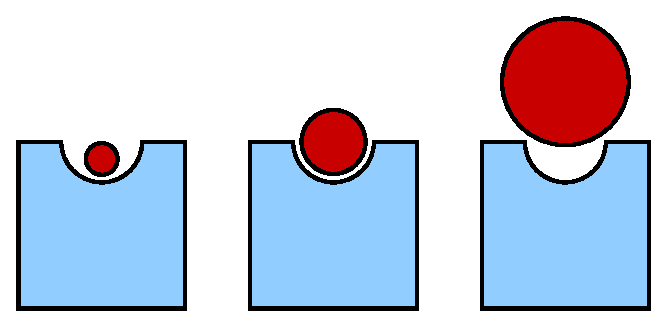
\includegraphics[width=\textwidth]{fig/binding-pocket}
		\caption{Binding-pocket volume}
		\label{fig:pocket-size}
	\end{subfigure}
	\hfill
	\begin{subfigure}[b]{0.45 \textwidth}
		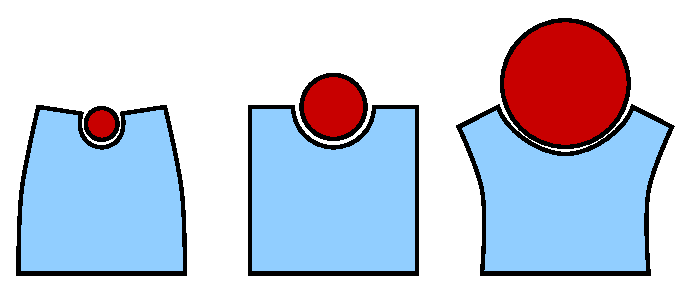
\includegraphics[width=\textwidth]{fig/binding-pocket-flex}
		\caption{Binding-pocket flexibility}
		\label{fig:pocket-flex}
	\end{subfigure}
	\caption{This figure shows different scenarios that may happen when an odorant molecule (ligand) binds to a receptor. 
		Fig. \ref{fig:pocket-size} shows the effect of binding-pocket volume. 
		From left to right, misfit because of small volume of molecule, perfect match and misfit because of large molecular volume.
		Fig. \ref{fig:pocket-flex} demonstrates that the flexibility of a receptor may compensate for the volume mismatches. 
		The red disks (dark grey in b\&w) are odorant molecule, 
		and the blue shapes (light grey in b\&w) are olfactory receptor and binding-pocket.}
	\label{fig:binding-pocket}
\end{figure}

Survival of many species depends on their olfactory system. 
They use it  to find food, 
avoid poison, 
escape from danger, 
mate, 
and bind to their offspring.
An olfactory system detects volatile chemicals in the surrounding, 
encodes the results and transmit them to limbic system and cortex.

The front end of the olfactory system are olfactory receptor neurons.  
Each neuron expresses only one kind of olfactory receptor (in insects they are co-expressed with Orco \cite{Larsson2004}),
neurons of the same type converge into the same glomeruli of the olfactory bulb (or antenatal lobe in insects),
so that each glomerulus of olfactory bulb receives an amplified signal from only one type of olfactory receptor~\cite{root2007,Carey2011,Vosshall2000,Couto2005,fishilevich2005,gao2000,wang1998,mombaerts1996,vassar1994}.
%That makes the olfactory bulb (or antennal lobe in insects) target of methods like calcium imaging (eg. ~\cite{Silbering2012}), 
%whereas electro-physiological studies directly target olfactory receptor neurons (eg.~\cite{Benton2010}). 

The olfactory systems use a combinatorial code: 
unlike many other receptors which are activated by only specific ligands (eq. neurotransmitters and hormones),
an olfactory receptor can be triggered by many odorant molecules, 
and an odorant molecule can interact different olfactory receptors~\cite{Malnic2000},

The combinatorial code helps the olfactory system to discriminates trillion odors~\cite{Bushdid2014}.
However, it is not clear yet which properties of a molecule contribute to its smell,
it is a topic of ongoing researches and there are many theories~\cite{Turin,Keller2004,Araneda2000,Brookes2007,Franco2011,Pelz2006,Gabler2013,Schmuker2007,Haddad2008,Snitz2013,Yablonka2012,gane2013}.

In this study, 
we investigate the relation between molecular volumes of odorants and the responses of olfactory receptor neurons. 
Our results suggest that molecular volume is a considerable factor, 
but not the only factor that determines the neural response of the olfactory receptor neurons.

The olfactory receptors are transmembrane proteins.
In vertebrates, they are metabotropic receptors, they belong to the family of g-protein coupled receptor (GPCR), 
Linda B. Buck and Richard Axel won the Nobel Prize in Physiology or Medicine, in 2004, 
for the discovery of this~\cite{Buck1991}.
There are many similarities between the olfactory system of insects and vertebrates~\cite{Wilson2014,Kaupp2010}, 
and it was assumed that insects use the same kind of signal transduction~\cite{Brody2000,Hill04102002}, 
but recently, it has been argued that the olfactory receptors in insects are inotropic~\cite{Sato2008,Wicher2008,Nagel2011,Rong2011}, 	
their topology is different from vertebrates~\cite{Benton2007,Smart2008},
and they function in presence of another common receptor, called Orco~\cite{Larsson2004}.


Regardless of the signal transduction, 
all olfactory receptor have the same function, they have a binding-pocket (also known as binding-cavity and binding-site),
where the ligands (odorants) bind to. 
Binding to an odorant activates receptors and 
the activated receptors changes the potential of the cell, 
directly (inotropic) or indirectly (metabotropic).

The amount of change in the membrane potential of an olfactory receptor neuron depends on the number of activated olfactory receptor proteins and the time that they remain activated,
which are determined by various physio-chemical properties of the ligand (odorant) and the receptor~\cite{Turin,Araneda2000,Gabler2013,guerrieri2005,uchida2000}, 
but here we focus only on two properties: the volume and the flexibility of the binding-pocket.
The molecular volume of a ligand should match the dimensions of the binding-pocket of the receptor,
then it fits into the binding-pocket of the receptor and triggers the signal transduction. 
Any mismatch in the volumes will affect the neural responses (Fig. \ref{fig:pocket-size}), 
on the other hand the flexibility of the binding-pocket can compensate for the volume mismatch (Fig. \ref{fig:pocket-flex}),

We could know the volume and flexibility of the binding-pocket, 
if we knew its three dimensional structure.
But this is not the case here, 
it is not easy to know the structure of integral proteins~\cite{Zhang2008,Lupieri2009}, 
including olfactory receptors. 
It is the topic of ongoing researches, 
using various methods like Molecular Dynamic (MD) simulations, 
mutagenesis studies, heterologus expression studies, and homology modeling~\cite{Khafizov2007,Man2004,Lai2005,Vaidehi2002,Floriano2004,Schmiedeberg2007,Katada2005,Kato2008,Rospars2013}.
In this study, we use neural recording to predict the {\it in-vivo} volume and flexibility of binding-pocket of olfactory receptors.

We suggest a functional relation between molecular volume and the neural responses, 
we provide a methodology to estimate {\it molecular receptive range} or {\it tuning function} of olfactory receptors,
and then we predict the structural properties of the binding-pocket of olfactory receptor - the volume and the flexibility of binding-pocket.
Our results may help to select odorants  for new experimental studies, 
may provide additional information about the structure of olfactory receptors to structural biologists, 
and may contribute to the study of olfactory coding.

To perform this study we use a public domain, 
well structured database -- DoOR -- 
that includes the neural responses of most olfactory receptors (OR) of Drosophila to many odorants~\cite{Galizia2010}. 
This database aggregated data from many sources~\cite{Bruyne1999,Bruyne2001,Dobritsa2003,Goldman2005,Hallem2004,Hallem2006,
Kreher2005,Kreher2008,Kwon2007,Pelz2006,Pelz2006,Schmuker2007,Stensmyr2003,
Turner2009,VanderGoesvanNaters2007,Yao2005}.

%%
%There are many studies that tries to connect physio-chemical properties of molecules to their perceived smells, like the current work, which studies the effect of molecular volume of odorants on the response of olfactory receptors.

%The olfactory system of insects are similar to the olfactory system of vertebrates in many ways ...  They are also differences .... 

%Some receptors respond to few molecules, some response to many.

%Insects receptors neurons show spontaneos activity of 8 Hz.

%Drosophila's olfactory receptors are ionotropic. They may be metabotropic. It is under debate.

% They have seven trans-membrane domains. They need Or83b to work. 
% they may construct a complex that work as a cation channel or Or83b functions as cation channel and collaborte with Olfactory receptor.

% Olfactory receptor are presents in other organs like kindny ans sperms.

%chemical receptory range.

%in GPCR odorant interact with helix 2,7
%2-58 candidate residues.

%Drosophila about 60 receptors, mamals 300-1300 receptors. 

%In low concentraiotn the response is narrow. In high concentration the response is broad.

%OR67d Pheremone. 
%Odor prediciton from the shape.
%Olfactory white.


%we show that the Drosophila melanogaster male-specific pheromone 11-cis-vaccenyl acetate (cVA) acts through the receptor Or67d to regulate both male and female mating behaviour. ~\cite{Kurtovic2007}
%we show that a Drosophila melanogaster CD36 homologue, Sensory neuron membrane protein (SNMP), is expressed in a population of olfactory sensory neurons (OSNs) implicated in pheromone detection.~\cite{Benton2007}
 
%we find that Drosophila ORs and OR83b adopt a novel membrane topology with their N-termini and the most conserved loops in the cytoplasm.~\cite{Benton2006}

%We find that major components of olfaction, including olfactory receptors (ORs), olfactory-related adenylate cyclase (AC3) and the olfactory G protein (G olf), are expressed in the kidney.~\cite{Pluznick2009}
 
%Most Drosophila olfactory neurons express two types of odorant receptor genes: Or83b, a broadly expressed receptor of unknown function, and one or more members of a family of 61 selectively expressed receptors.~\cite{Larsson2004}
 
%Humans can discriminate several million different colors and almost half a million different tones,On the basis of the results of psychophysical testing, we calculated that humans can discriminate at least 1 trillion olfactory stimuli.~\cite{Bushdid2014}

\section*{Material and methods}
\begin{figure}
	\centering
	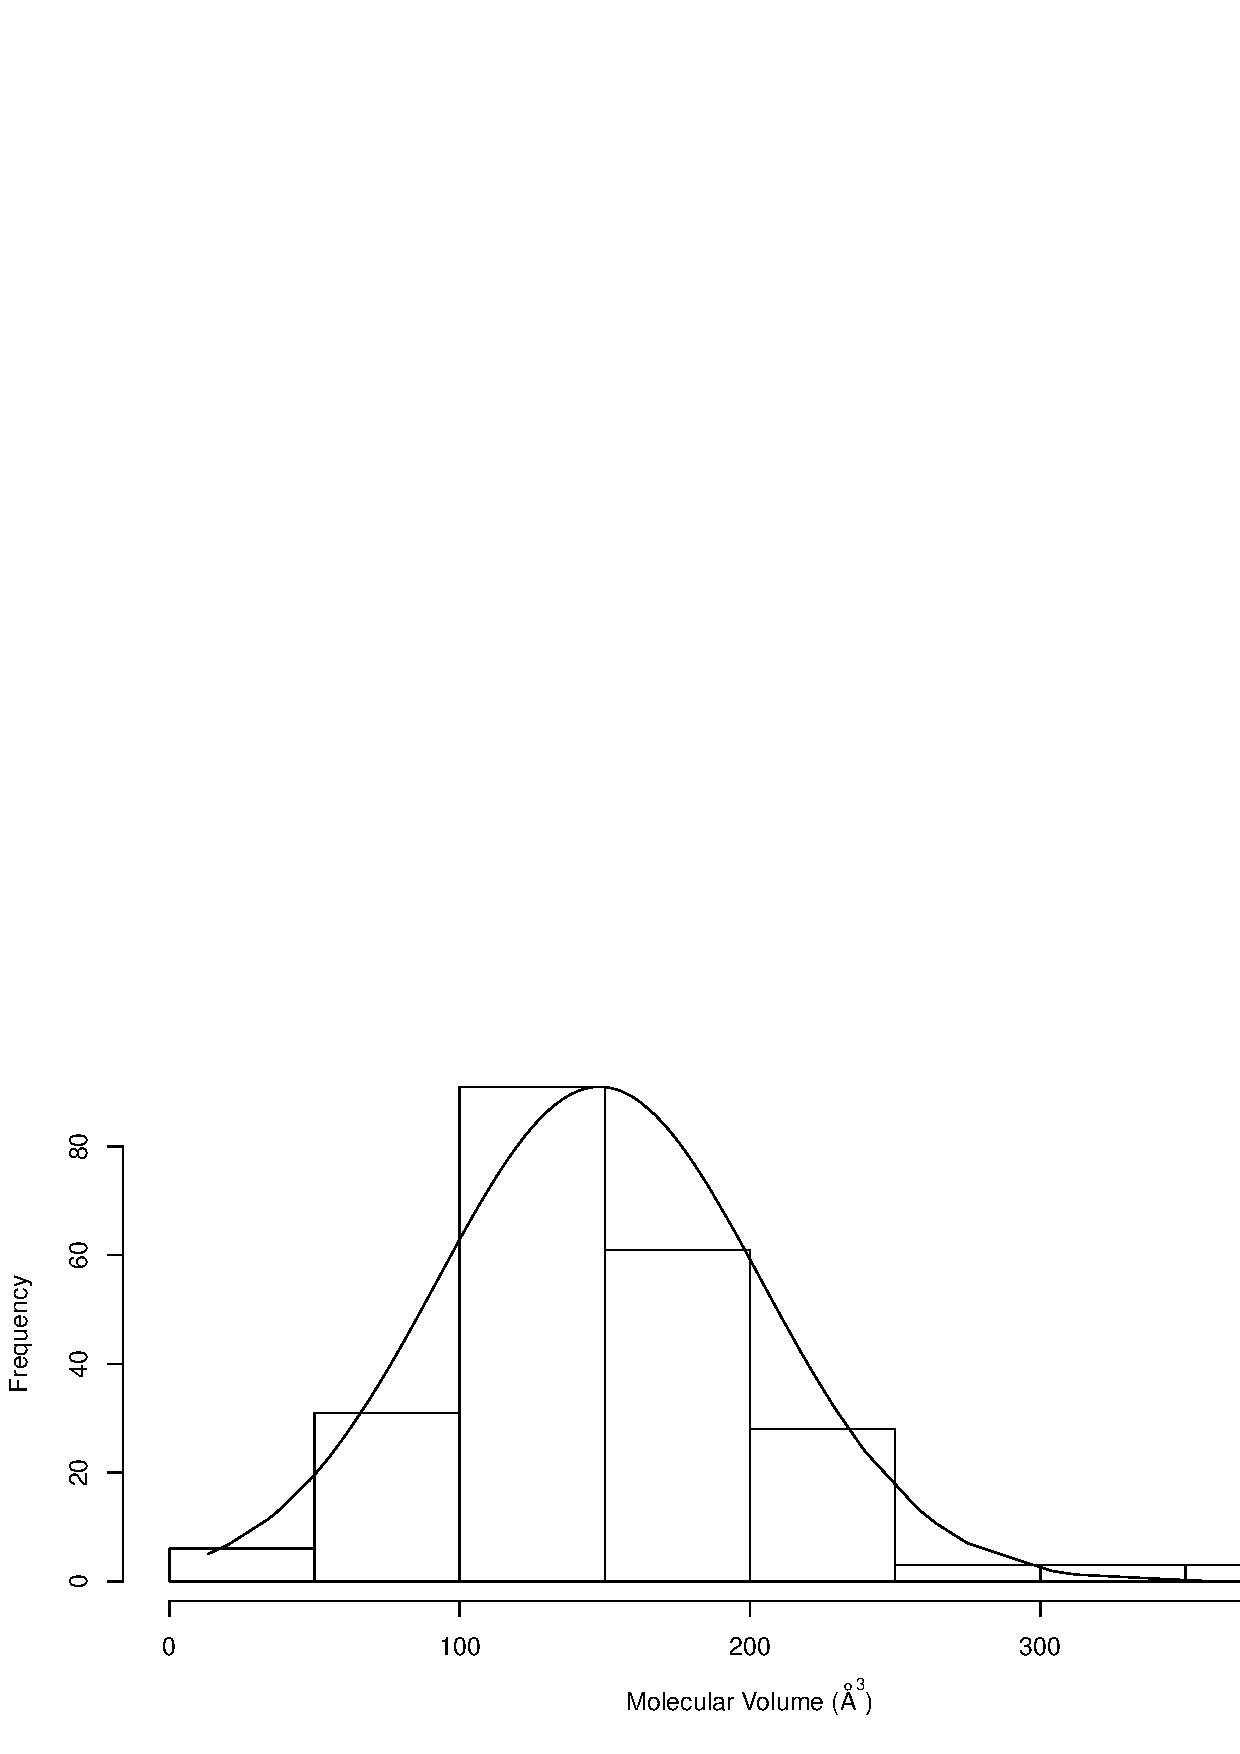
\includegraphics[width=0.5 \textwidth]{fig/hist-volumes}
	\caption{Density function of molecular volumes $g(v)$, considering all molecules of DoOR database. 
		%The actual density function of molecular of volumes in each experiment, $g(v)$, might be slightly different  because each experiment uses a different subset of molecules. 
		The solid line is a Gaussian fit (Eq. \ref{eqn:hist-volumes}) and the dashed line shows the median, 
		which is slightly different from  the mean.}
	\label{fig:hist-volumes}
\end{figure}

We want to study the relation between neural responses and molecular volumes, 
so we need the respective data. 
We take the neural data of DoOR database \cite{Galizia2010} and we calculate molecular volume (supplemental file 3) using a computational chemistry software -- VEGA ZZ~\cite{Pedretti2004}. 
We used  GNU R to analyze the data~\cite{Rlanguage}.

DoOR database can be summarized in an $N\times M$ matrix. 
Its elements, $r_{nm}$, are the response of neuron $n$ to odorant $m$. 
This matrix is normalized between 0 and 1 so we have $0 \le r_{nm} \le 1$, where 1 is the strongest response.
The only problem is that this matrix has many {\it Not Available} (NA) values, 
and different neurons are excited by different set of odorants, 
so  when summing over $m$, $\sum_m$, we are calculating $\sum_{m: r_{nm} \neq \text{NA}}$, 
but for simplicity, 
we use the former notation. 

The response $r_{nm}$ depends on the molecular volume of the odorant, $v_m$, 
and other physio-chemical properties of the molecule $m$; 
We assume that we can separate the response $r_{nm}$ into two terms:

\begin{equation}
	r_{nm} = f_n(v_m) \psi_{nm}.
	\label{eqn:factors}
\end{equation}
The first term, $f_n(v_m)$, depends only on the molecular volume of odorants.
The second term, $\psi_{nm}$ include every other influential properties of molecules, but the molecular volume.
Both terms are characteristic of each receptor, and they might vary from neuron to neuron.
In fact, the first term, $f_n(v)$, is the tuning curve of neuron $n$ in respect to the molecular volumes, 
it can be approximated with a Gaussian function

\begin{equation}
	\displaystyle f_n(v) = e^{-\frac{(v-v_n)^2}{2\sigma^2_n}}, 
	\label{eqn:volume-dependence}
\end{equation}
where, $v_n$ is the preferred molecular volume of receptor $n$ and $\sigma_n$ represents its flexibility. 
In this work we want to estimate $v_n$ and $\sigma_n$. 
To do so, first we calculate the response weighted average of molecular volumes, 
$\frac{\sum_{m} v_m r_{nm}}{\sum_{m} r_{nm}}$ and then we use (\ref{eqn:factors}):

\begin{equation}
	\frac{\displaystyle \sum_{m} v_m r_{nm}}{\displaystyle \sum_{m} r_{nm}} = \frac{\displaystyle \sum_{m} v_m f_n(v_m) \psi_{nm}}{\displaystyle \sum_{m} f_n(v_m) \psi_{nm}}.
	\label{eqn:sta}
\end{equation}
Here we can approximate $\sum$ with $\int$, which is common in statistical physics:

\begin{equation}
	\sum_{m} \dots f_n(v_m) \psi_{nm} \approx  \langle \psi_{nm} \rangle_m \int_0^\infty \dots f_n(v) g(v)  dv. 
	\label{eqn:sigma_to_int}
\end{equation}
In which, 
$\langle \psi_{nm} \rangle_m$ denotes the average of $\psi_{nm}$ over all $m: r_{nm} \neq \text{NA}$. 
It can be moved out of the integral for it is independent of $v$.
In the above equation, 
$g(v)$ is the density of states, $g(v) dv$ indicates how many molecules have a molecular volume in the range of $v$ and $v+dv$.
This function can be approximated by a Gaussian function, Fig.\ref{fig:hist-volumes}, 

\begin{equation}
	g(v) = e^{-\frac{(v- v_{g})^2}{2 \sigma_{g}^2}},
	\label{eqn:hist-volumes}
\end{equation}
ideally, $g(v)$ should not depend on the neuron $n$, 
it is the property of ensemble of odorant molecules, not neurons. 
But here, we have many missing values ($r_{nm} = NA$), 
so we have to calculate $g(v)$ for each neuron separately; 
Therefore, $v_{g_n}$ and $\sigma_{g_n}$ are the average and standard deviation of molecular volume while $r_{nm} \neq \text{NA}$.
Now we rewrite equation (\ref{eqn:sta}) using equation (\ref{eqn:sigma_to_int}):

\begin{equation}
	\frac{\displaystyle \sum_{m} v_m r_{nm}}{\displaystyle \sum_{m} r_{nm}} \approx \frac{\displaystyle \int v f_n(v) g_n(v) dv}{\displaystyle \int f_n(v) g_n(v) dv}.
	\label{eqn:sta_int}
\end{equation}
We replace the product of $f_n(v)$ and $g_n(v)$ in the above equation with $h_n(v) = f_n(v) g_n(v)$, to make a simpler form

\begin{equation}
	\frac{\displaystyle \sum_{m} v_m r_{nm}}{\displaystyle \sum_{m} r_{nm}} \approx \frac{\displaystyle \int_v v h_n(v) dv}{ \displaystyle \int_v  h_n(v) dv }.
	\label{eqn:mean}
\end{equation}
The function $h_n(v)$ is a Gaussian function because it is the product of two Gaussian functions, 

\begin{equation}
h_n(v) = e^{-\frac{(v-\mu_{h_n})^2}{2\sigma_{h_n}^2}}, 
\end{equation}
so the right hand side of equation \ref{eqn:mean} is nothing but $\mu_{h_n}$ and 
in a similar way, we can calculate $\sigma_{h_n}$ from the neural data

\begin{eqnarray}
	\mu_{h_n} &\approx& \frac{\displaystyle \sum_{m} v_m r_{nm}}{\displaystyle \sum_{m} r_{nm}} \\
	\sigma_{h_n}^2 &\approx& \frac{\displaystyle \sum_{m} v_m^2 r_{nm}}{\displaystyle \sum_{m} r_{nm}} - \mu_{h_n}^2
	\label{eqn:final_h}
\end{eqnarray}•


We knew the mean $v_{g_n}$ and standard deviation $\sigma_{g_n}$ of $g_n(v)$ from the molecular volumes of the ensembles of odorants. 
We just calculated the mean $\mu_{h_n}$ and standard deviation $\sigma_{h_n}$ of $h_n(v)$ from the neural data.
Now calculating the mean $v_n$ and the standard deviation $\sigma_n$ of $f_n(v)$ is trivial,
first we calculate $\sigma_n$ from 

\begin{equation}
	\frac{1}{\sigma_n^2} = \frac{1}{\sigma^2_{h_n}}  - \frac{1}{\sigma^2_{g_n}}
\end{equation}•
and then we calculate $v_n$: 

\begin{equation}
	\frac{v_n}{\sigma_n^2}  =    \frac{\mu_{h_n}}{\sigma^2_{h_n}} - \frac{v_{g_n}}{\sigma^2_{g_n}}.
\end{equation}•
The calculated $v_n$ and $\sigma_n$ are in supplemental file 1. 
The resulting $f_n(v)$ are plotted over the actual data, for \numberofreceptors receptors (Fig.~\ref{fig:vol-res}),
in which p-values $<0.05$. 

We calculate p-values by permutation test. 
The alternative hypothesis is 
``{\it The response of olfactory receptor neurons depend on the molecular volume of odorants.}'', 
which require  a finite value for $\sigma_n$, 
then the null hypothesis is 
``{\it The response of olfactory receptor neurons is independent of molecular volume of odorants.}'',
which require $\sigma_n \rightarrow \infty$, 
so p-value is the probability of having $\sigma'_n\leq\sigma_n$, 
where $\sigma_n$ is calculated from the original data, but $\sigma'_n$ calculated using permuted version.

We are testing a hypothesis on  $\sim$60 olfactory receptors simultaneously. 
If we use a simple threshold of 0.05 for the p-value of each receptor, we may have false positives. 
To address this issue, multiple-comparison problem, 
we use Bonferroni correction. 
The problem with Bonferroni correction is that it may increases false negatives.
This problem can be addressed using another method -- False Discovery Rate (FDR).
We used both methods -- Bonferroni and FDR, as well as no correction. 
The result are labeled accordingly in Fig.\ref{fig:vol-res}.

We also wants to show that the diversity of volume and flexibility of binding pocket among receptors.
To estimate the p-values, 
we take any pair of receptors that was sensitive molecular volume (\numberofreceptors receptors),
calculate their difference, 
use a permutation test and measure the probability of having them to be that different only by chance.
The results are in Fig.~\ref{fig:p-values}.

%Now we know the preferred volume $v_n$ of each receptor and also its flexibility $\sigma_n$.


\section*{Results and discussions}
\begin{figure}
	\centering
%	\begin{subfigure}[b]{\textwidth}
		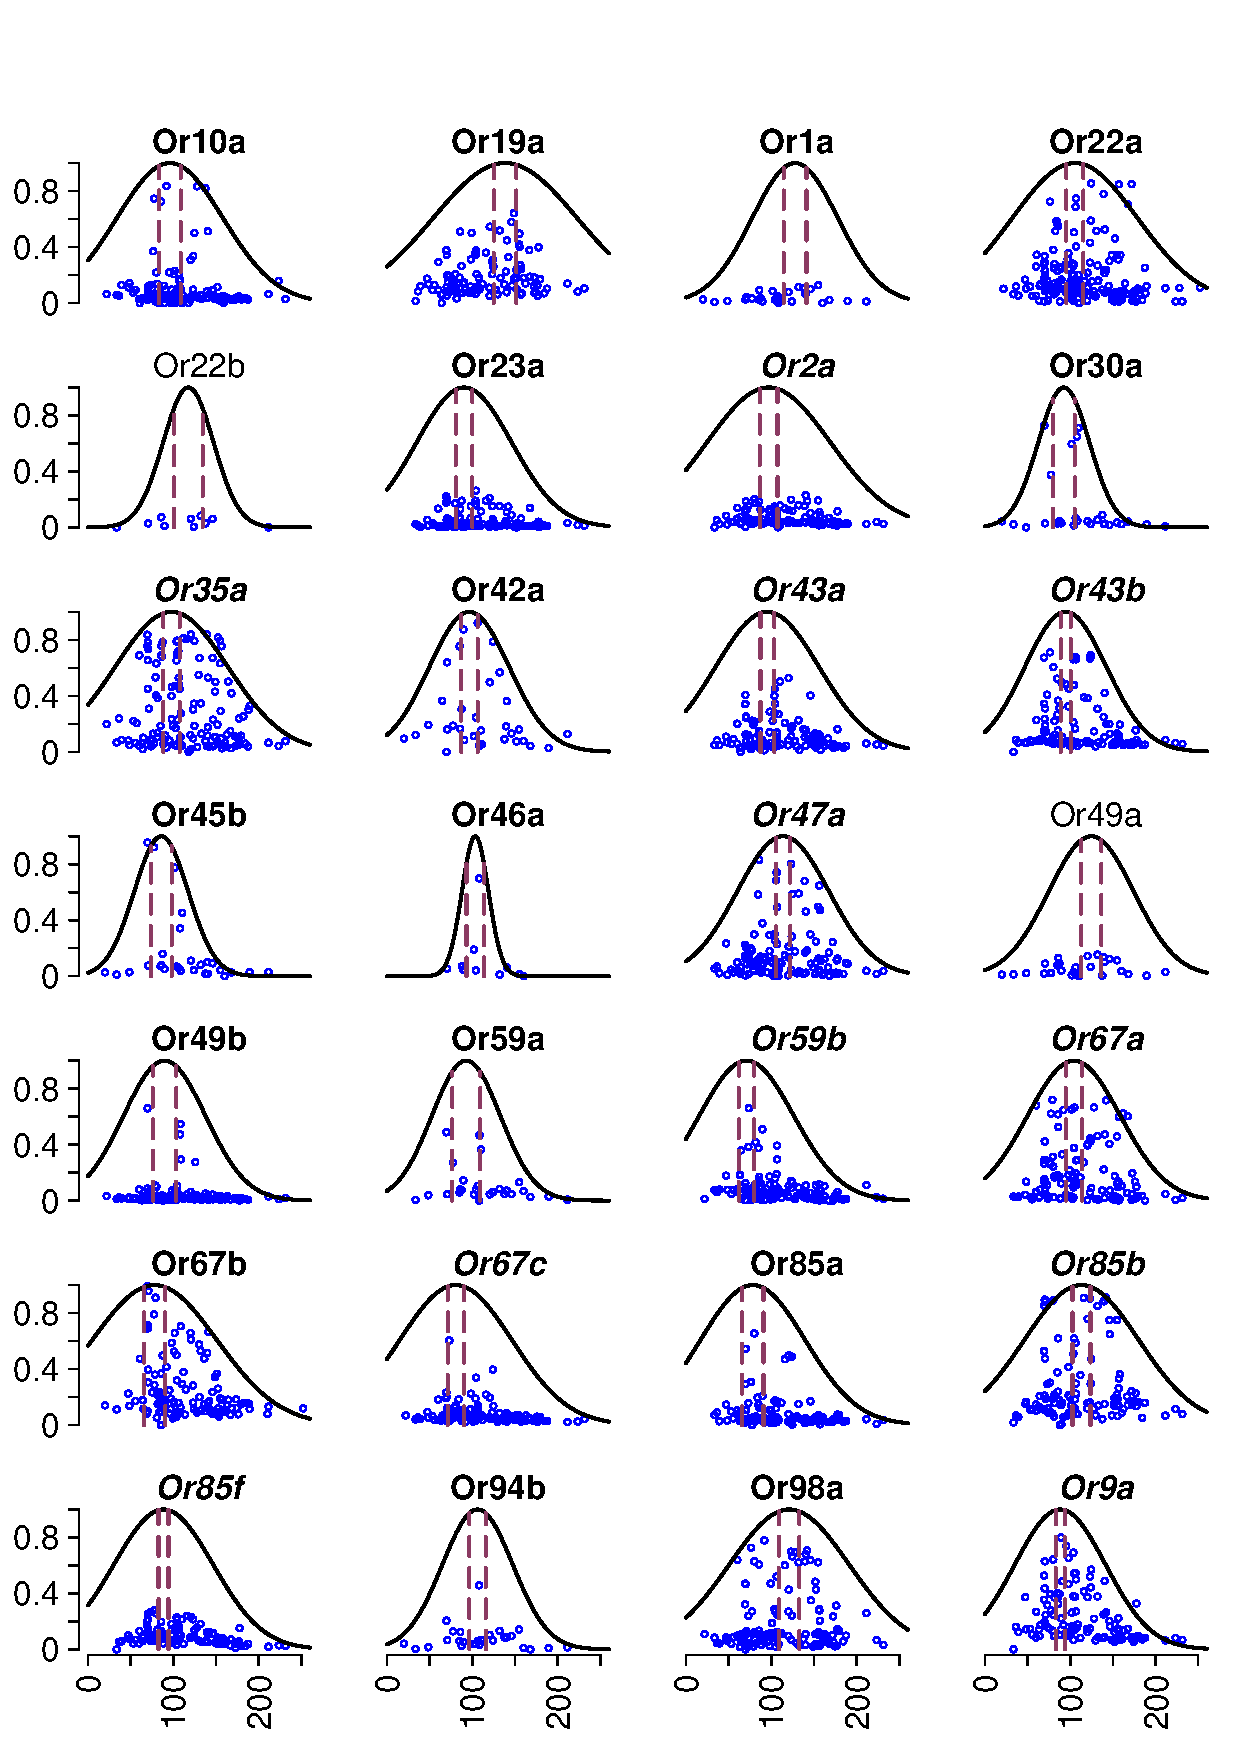
\includegraphics[width=0.8 \textwidth]{fig/vol-res-}
		%\caption{}
		\label{fig:vol-res:all}		
%	\end{subfigure}
%	\begin{subfigure}[b]{0.75 \textwidth}
%		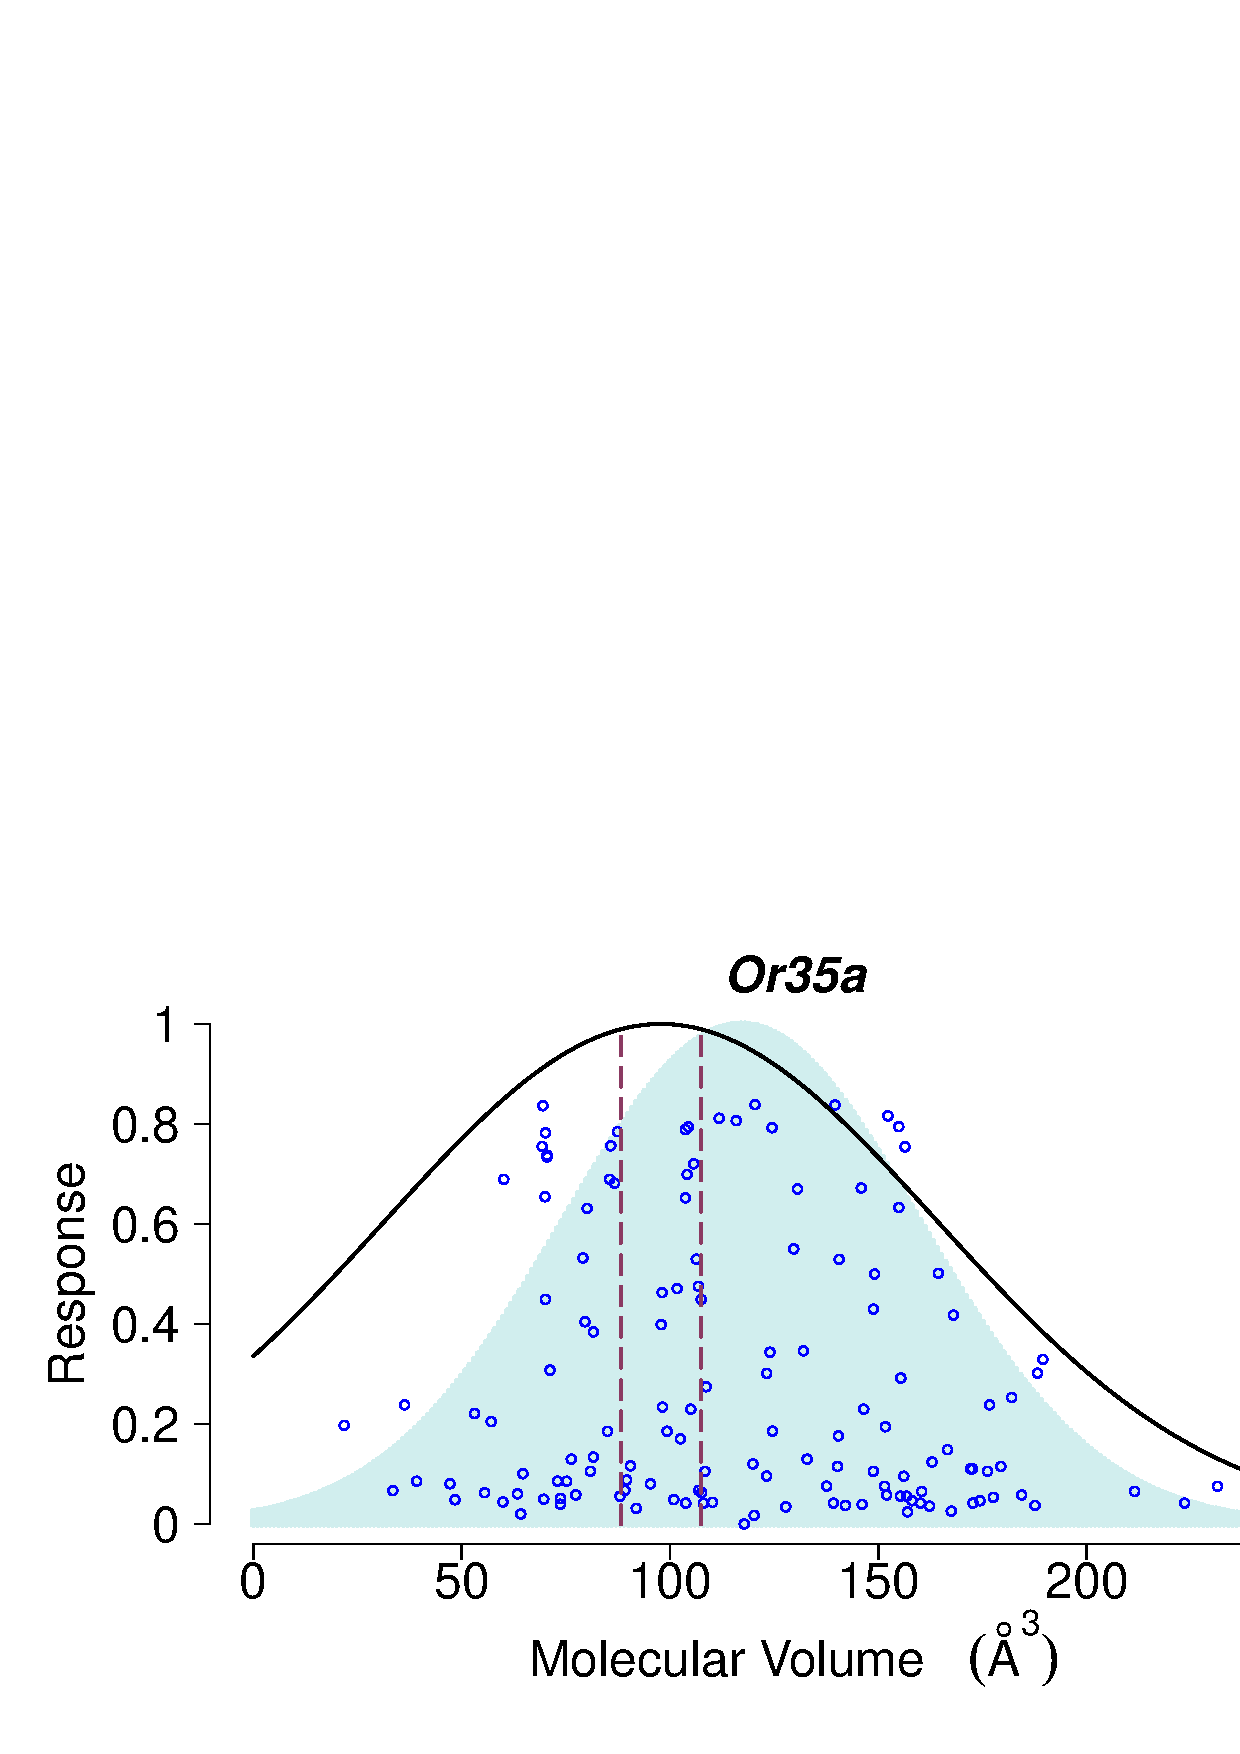
\includegraphics[width= \textwidth]{fig/vol-res-Or35a}
%		\caption{}	
%		\label{fig:vol-res:one}	
%	\end{subfigure}
	\caption{Response of olfactory receptors  versus molecular volume of odorants (circles),  
			the fitted functions $f_n(v)$ from Eq.~\ref{eqn:factors} (solid lines), 
			and the error bars of the mean of $f_n(v)$ (red vertical lines), 
			for \numberofreceptors receptors that their response showed significant (p-value $<0.05$) dependence to molecular volume. 
			Among them, \fdr are significant according to FDR correction (receptor names in bold) and 
			\bonferroni are significant considering Bonferroni correction (receptor names in italic).
		}
	\label{fig:vol-res}
\end{figure}

\begin{figure}
%	\begin{subfigure}[b]{\textwidth}
		\centering
		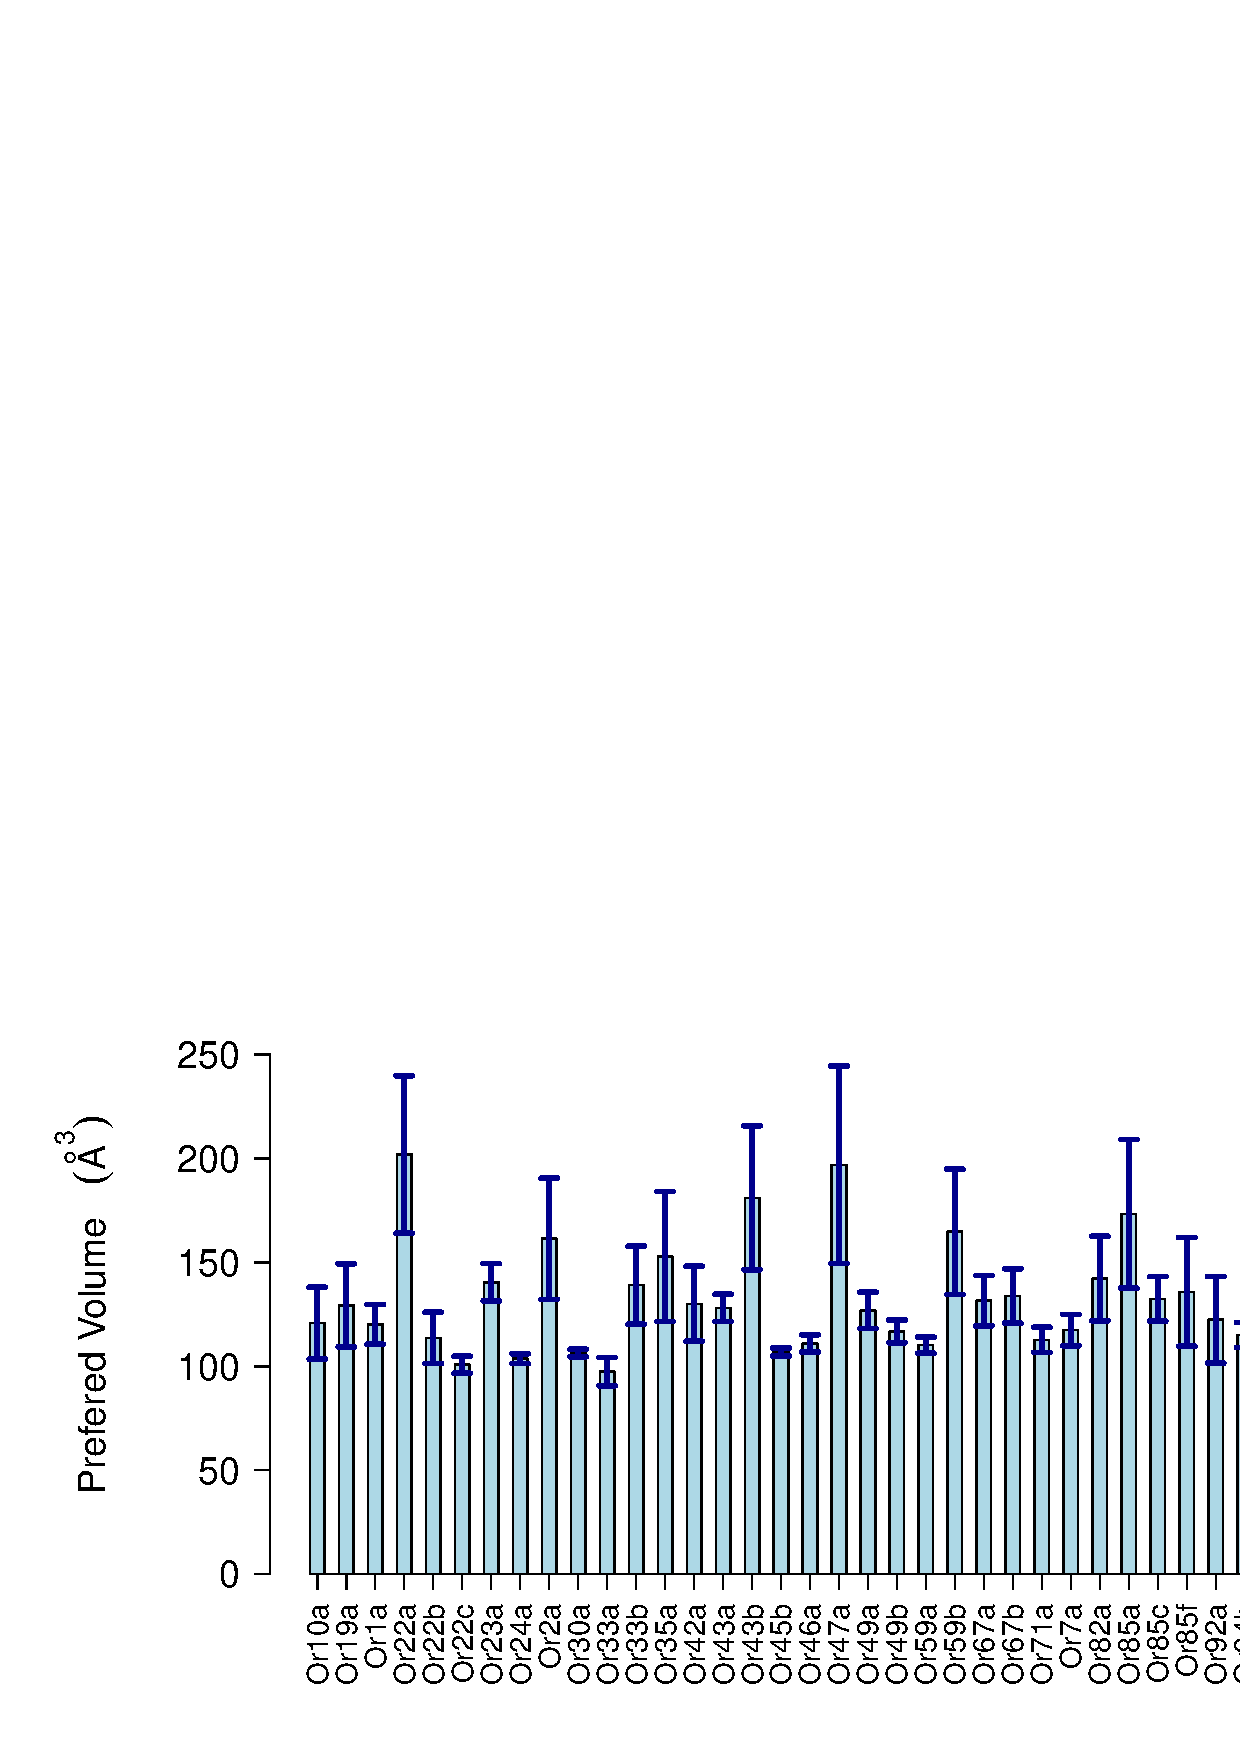
\includegraphics[width=  0.85 \textwidth]{fig/mean-vol}
		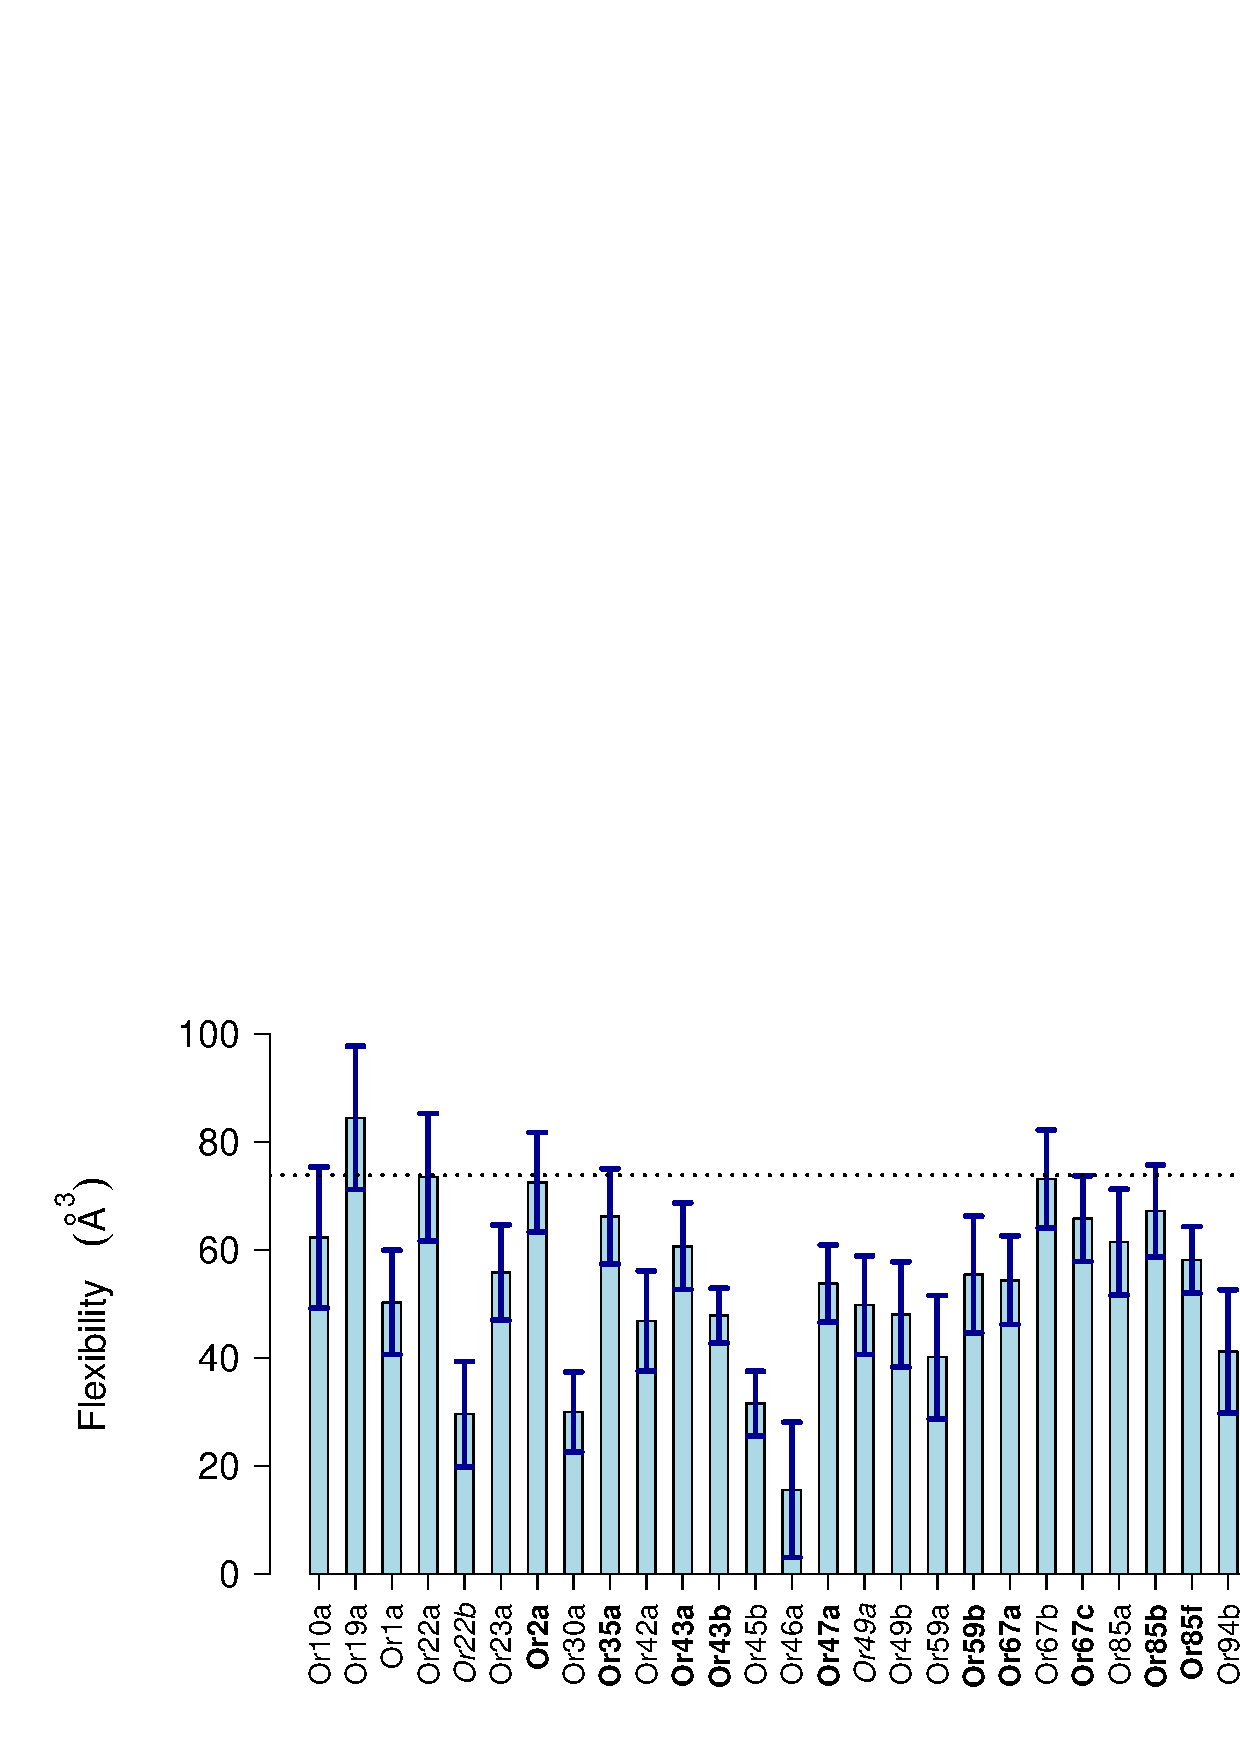
\includegraphics[width=  0.85 \textwidth]{fig/std-vol}
%	\end{subfigure}
	\caption{The preferred volumes of \numberofreceptors receptors $v_n$ (top). 
		and their flexibilities $\sigma_n$ (down). 
		The error bars are calculated using Jack-Knife method. 
		Some receptors like Or59b, Or67a and  Or85a prefer smaller molecules, 
		but some others like Or19a,  Or1a and  Or49a prefer larger molecules.
		Some receptors like Or46a,  Or22b and Or30a are volume  selective, 
		but some others like Or19a,  Or67b and  Or22a respond to broader range of molecular volumes.
		}
		\label{fig:preferred_volume}
		\label{fig:volume_flexibility}
\end{figure}


\begin{figure}
% do not touch this fig.
	\centering
	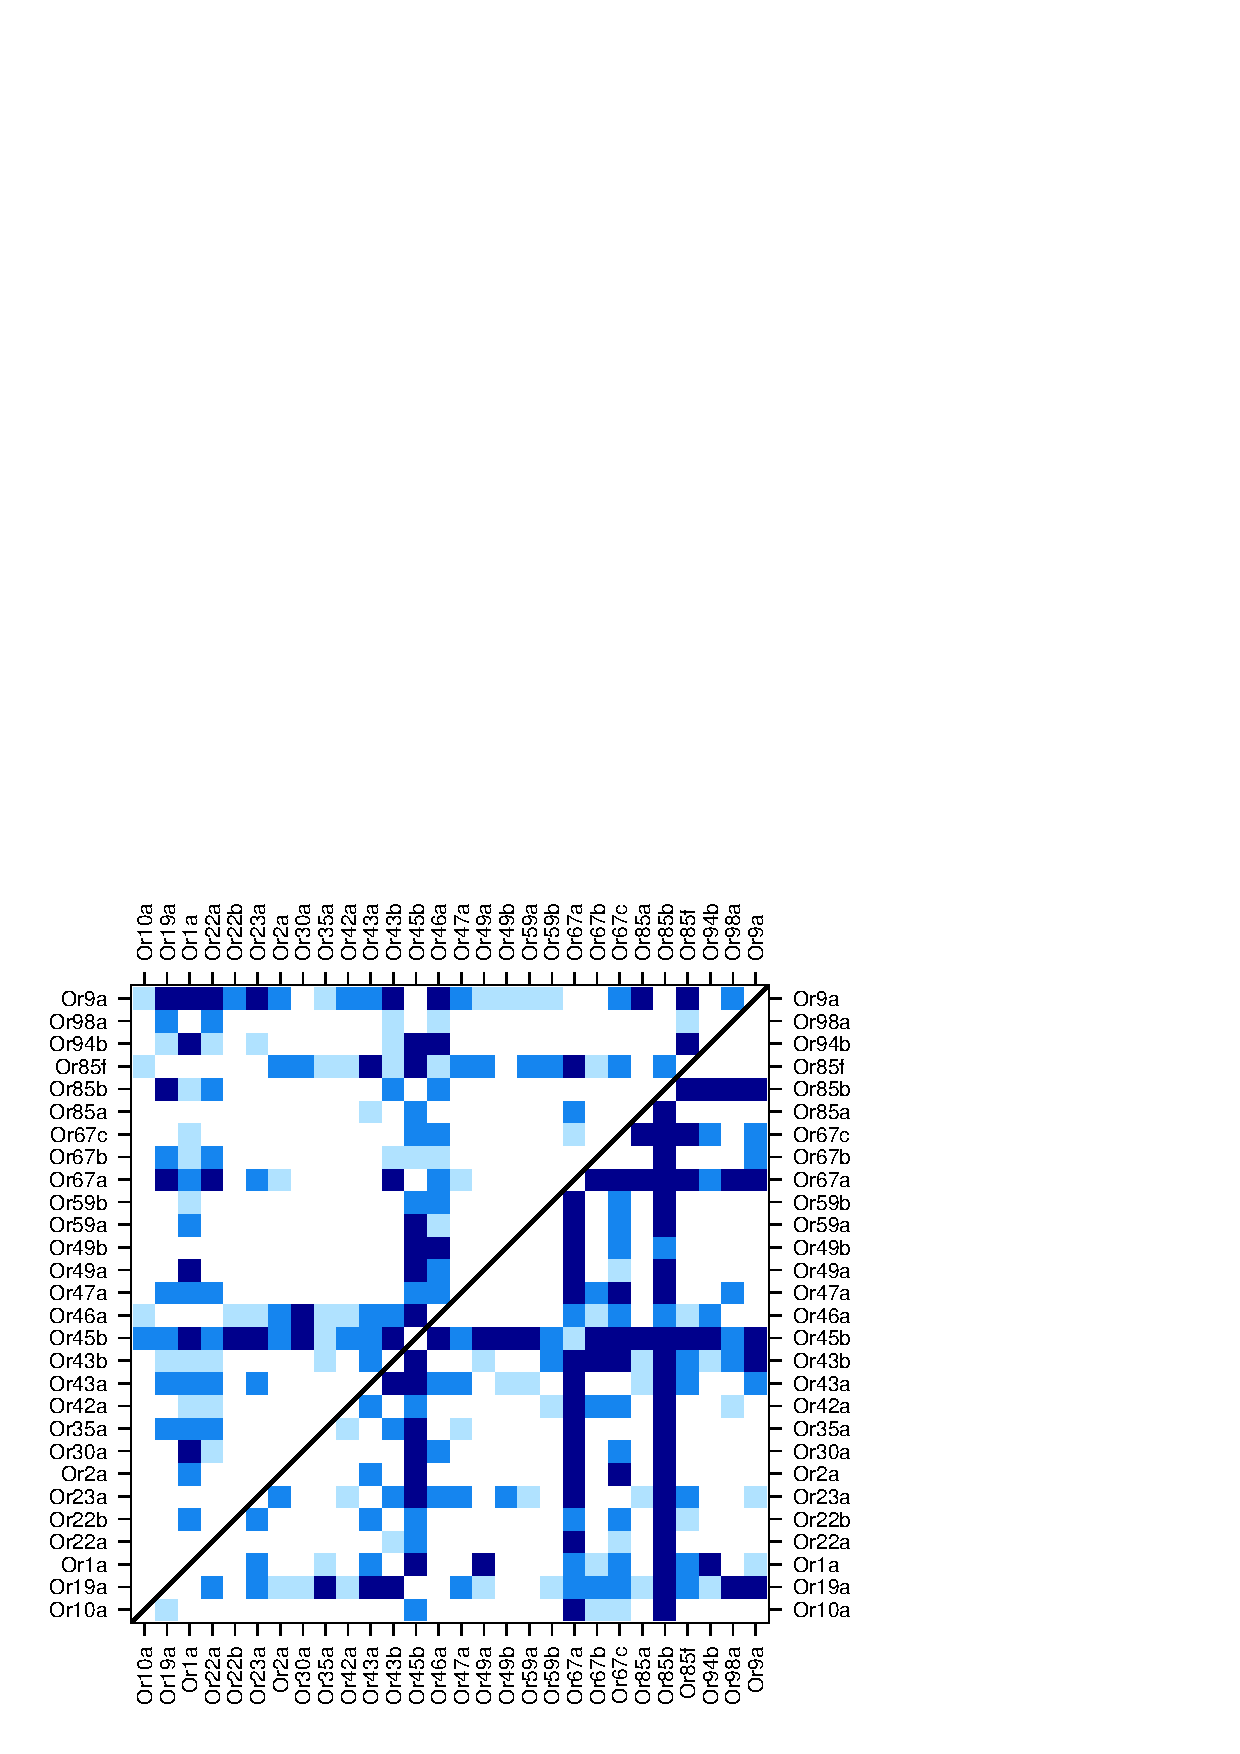
\includegraphics[width= 0.5 \textwidth]{fig/pair-pval}
	\caption{Pairs of olfactory receptors that differ significantly in their binding-pocket's volume (upper triangle) and flexibility (lower triangle).
			All blue shades have p-value of less than 0.05, 
			two darker shades have FDR corrected p-values of less than 0.05 and the darkest shade has Bonferroni corrected p-value of less than 0.05.}
	\label{fig:p-values}
\end{figure}

There are two main assumption in this work: 
First we assumed that the response of an olfactory receptor can be factorized into two terms, 
according to (\ref{eqn:factors}).
Second, we assumed that the volume dependence factor $f_n(v_m)$ in (\ref{eqn:factors}) 
have a Gaussian form (Eq. \ref{eqn:volume-dependence}).
Considering the physics and chemistry behind the binding-process (Fig. \ref{fig:binding-pocket}), 
and the neural responses (Fig. \ref{fig:vol-res}), 
these assumptions are logical. 

%but, to be sure, we also put them in a test. 
%After calculating function $f_n(v)$ for each olfactory receptor, we can calculate $\psi_{nm}$ of the equation \ref{eqn:factors}.
%If $\psi_{nm}$ is independent of molecular volumes, it means that the assumptions where justified.

The function $f_n(v)$ can be considered as the tuning curve of olfactory receptor $n$ in response to molecular volume (Fig.~\ref{fig:vol-res}). 
Each receptor has a preferred molecular volume $v_n$ and shows some flexibility $\sigma_n$, 
The calculated $f_n(v)$ are in  Fig.~\ref{fig:vol-res}, 
it includes \numberofreceptors receptors, 
which show a significant dependence to molecular volume of odorants in their response (p-value $<0.05$).

To address the multiple comparison problem, 
we also calculated the level of significance according to both Bonferroni (very conservative) and FDR (less conservative) corrections. 
From the results of \numberofreceptors receptors, 
\bonferroni of them are significant according to Bonferroni correction (receptor names in italic), 
\fdr of them are significant according to FDR correction 
(receptor names in bold), 
and the rest (\nocorrection receptors), 
only satisfy the criteria of  p-value $<0.05$, without any corrections.
Considering the FDR correction, 
we can conclude that close to half of receptors (\fdr / 60 ) show significant sensitivity toward molecular volumes. 
The other half could be sensitive to molecular volume as well, but the current evidence are not enough and
more experiments are necessary.
%\begin{table}
%\begin{center}
%    \begin{tabular}{ | l | l | l |l |}
%    \hline
%     &  $p_{value} < 0.05$ & FDR & Bonferroni \\ \hline
%     {\small Receptors are sensitive to molecular volume} &  28 &  26 & 11\\ 
%     $v_{n_1} = v_{n_2}$&  21 & 23 & 38\\ \hline
%    \end{tabular}
%\end{center}
%\caption{Times that the null hypothesis has been rejected, according to different method}
%\end{table}
The parameters of $f_n(v)$, $v_n$ and $\sigma_n$ are in Fig. \ref{fig:preferred_volume}.
Figure \ref{fig:preferred_volume} demonstrate that the molecular volume preference of receptors are different (top). 
and the flexibility of receptors are also different (bottom).
To back these claims, 
we estimated the p-values of having different volume preference and flexibility for each pairs of \numberofreceptors receptors
(Fig.~\ref{fig:p-value}). 
From all possible 378 pairs, 
when comparing the volume preferences, 
133 have a p-value of less than 0.05, 
this number reduces to 89 after using FDR and further reduces to 32 using Bonferroni correction.
When comparing flexibilities, 
the numbers become 168, 134 and 77 respectively. 
The union of these two set says that 226 (p-value $<0.05$), 171 (FDR corrected), and 91 (Bonferroni corrected) pairs of receptors showed distinct differences in their binding-pocket characteristics.

This diversity is important in perceiving the quality of smells. 
In a hypothetical experiment, 
assume that every characteristic of odorant molecules are the same but their molecular volume.
If all olfactory receptors had the same preferred volume and flexibility, 
any change in the molecular volume would change only the intensity of smell not its quality.
But olfactory receptors have different preferred volumes and flexibilities, 
so any change in the molecular volume of an odorant results in a different combinatorial encoding which affects the quality of perceived smell as well its intensity.
This agrees with the work of M. Zarzo: larger molecules  smell better~\cite{zarzo2011}.
That may describe the difference in the smell of methanol, ethanol, propanol and butanol. 
Methanol smells pungent, ethanol smells pleasant and winy, propanol and butanol smell like ethanol except butanol  has a little banana like aroma.
The molecular volume affects the combinatorial encoding, 
and the combinatorial code determines the quality of odorants.

Here we showed that the responses of olfactory receptor neurons are related to the molecular volume of odorants, 
apart from that, it is not clear which other features of molecules are measured by olfactory receptors. 
It is a topic of ongoing researches, 
there are many works that try to connect the physio-chemical properties of molecules to the evoked neural response or perceived smells.
But the non-linear volume dependence (Eq. \ref{eqn:factors} and Eq. \ref{eqn:volume-dependence})  
may mask important relations between molecules and neural responses.

By considering the effect of molecular volume on the response of olfactory receptor neurons, 
one might discover more subtle dependence between other molecular features and neural responses, 
by investigating $\psi_{nm}$, 
which otherwise would be masked by this non-linear relation $f_n(v)$.

We also predict some {\it in-vivo} structural aspects of  the binding-pocket of olfactory receptors:
the preferred volume of each receptor results from the volume of the binding-pocket,
the flexibility of a receptor results from the rigidity or flexibility of the binding-pocket; 
%Therefore, our results provides information about both structural and dynamical properties of olfactory receptors in Drosophila. 
These data add some constrains over the 3d structure of olfactory receptors, 
which may help the prediction and calculation of 3d structure of these proteins. 

The method of this work can be combined with mutagenesis as well. 
Some genes of an olfactory receptor are mutated, 
then its response to a selection of molecules are measured and finally the preferred volume and flexibility are calculated.
In this way we can understand which amino acids of the olfactory receptor contribute to the volume and flexibility of the binding-pocket, 
as well as affecting the function of the receptors.

Our finding can also save time and expenses of experiments by suggesting important odorants for each receptor.
To study $\psi_{nm}$ of a receptor, 
it is better to have many data points and those data points are better to be around the preferred volume of the receptor.
But this is not the case in current data, 
for many receptors, 
most data points are on the tails of $f_n(v)$, which is close to zero.
We have suggested the best selection of odorants for each of \numberofreceptors studied receptors 
(see Venn diagram in Fig.~\ref{fig:odorant-suggest} and supplemental file 2).

\begin{figure}
\centering
	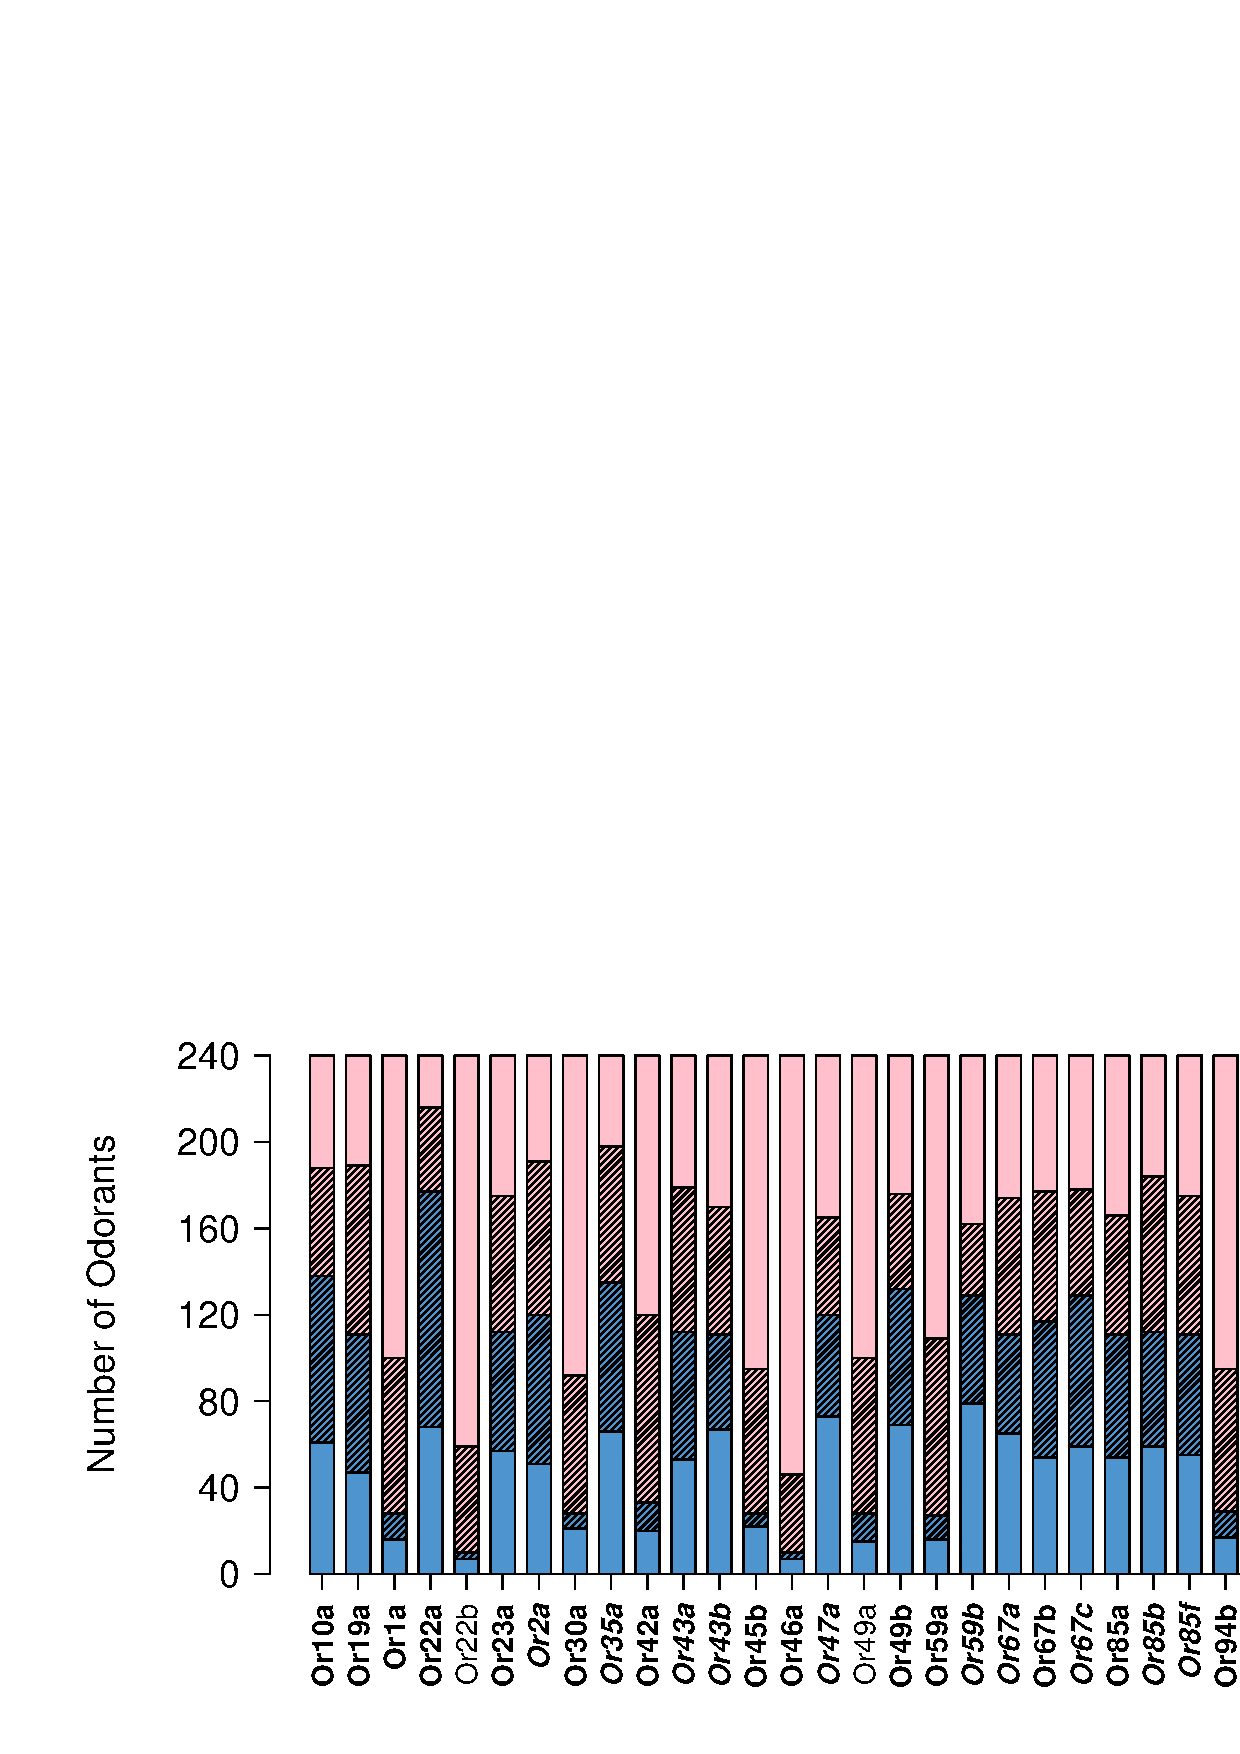
\includegraphics[width=\textwidth]{fig/odorant-suggest}
	\caption{Venn diagram of DoOR database and our suggested important odorants of each receptor.
			The database includes 240 molecules, 
			some are used to study an olfactory receptor (blue areas), 
			and data for the rests are not available (pink).
			The hatched area are odorants with molecular volume close to the preferred volume of each receptor
			($v_n \pm \frac{\sigma}{2}$).
			We already know the neural response of hatched blue areas, 
			but the hatched pink odorants could be the target of future experiments, we predict the rest give only zeros.
			}
	\label{fig:odorant-suggest}
\end{figure}

Although this work is on the data of Drosophila, 
we expect that the general principles and methodologies of this work hold for vertebrates as well. 
But considering the similarities and dissimilarities between insects and vertebrate, 
this should be verified.

Approximating $f_n(v)$ and $g(v)$ with a Gaussian function makes the mathematical formulation simple and readable. 
But a semi-infinite function may be a better choice for molecular volumes can not have negative values.

\section*{Acknowledgments}
We are especially grateful to B. N. Araabi, S. Aghvami and N. Doostani for the careful reading of the manuscript; and P. Carloni for the fruitful discussion.

%\printbibliography

\bibliography{binding-pocket}

\bibliographystyle{Science}


\end{document}
